\documentclass[11pt]{article}
\usepackage[margin=1in]{geometry}
\usepackage{graphicx}
\usepackage{booktabs}
\usepackage{siunitx}
\usepackage{amsmath}
\usepackage{hyperref}
\usepackage{caption}
\usepackage{subcaption}
\usepackage{float}

\title{Spectroscopic Ellipsometry Analysis\\
Cap\_01242007 Dataset: Ta\textsubscript{2}O\textsubscript{5} on Ta Metal}
\author{Jovan Trujillo\\
Advanced Electronics and Photonics Core\\
Arizona State University}
\date{January 24, 2007}

\begin{document}
\maketitle

\section{Introduction}

This report presents the spectroscopic ellipsometry (SE) analysis of tantalum oxide
(Ta\textsubscript{2}O\textsubscript{5}) thin films deposited on tantalum metal substrates.
Six wafers from the Cap\_01242007 dataset were analyzed using an optical model developed
in collaboration with Neha Singh.

The optical constants for the tantalum metal substrate were obtained using a point-by-point
(PBP) fit to the original tantalum metal data (ta\_pbp.mat). Barry O'Brien performed
the optical constant fit using an aluminum model, which produced sufficiently smooth
data for reliable fitting.

\section{Optical Model}

The layer structure used for fitting is:

\begin{center}
\begin{tabular}{cl}
\toprule
Layer & Description \\
\midrule
Ambient & Air ($n = 1.0$) \\
Film & Ta\textsubscript{2}O\textsubscript{5} (Cauchy dispersion) \\
Interface & EMA (Ta\textsubscript{2}O\textsubscript{5} + Void) \\
Substrate & Ta metal (PBP optical constants) \\
\bottomrule
\end{tabular}
\end{center}

\subsection{Cauchy Dispersion for Ta\textsubscript{2}O\textsubscript{5}}

The transparent Ta\textsubscript{2}O\textsubscript{5} film is modeled with a Cauchy dispersion:
\begin{equation}
n(\lambda) = A + \frac{B}{\lambda^2} + \frac{C}{\lambda^4}
\end{equation}
where $\lambda$ is in micrometers. The extinction coefficient $k = 0$ in the fit range
(\SI{320}{}--\SI{1698}{nm}).

\subsection{EMA Interfacial Layer}

An Effective Medium Approximation (EMA) layer between the Ta\textsubscript{2}O\textsubscript{5}
and Ta metal represents the porous interface created during the oxidation reaction. The EMA
mixes Ta\textsubscript{2}O\textsubscript{5} optical constants with voids (air, $n = 1.0$).

This interfacial layer is attributed to surface roughness from the columnar grain structure
of the tantalum metal. The different mobility of ions during oxidation creates an interface
where the stoichiometry differs from the bulk film. Note that substituting surface roughness
(srough.mat) for void.mat produces statistically identical results, consistent with this
interpretation.

\subsection{Fitting Procedure}

The fitting was performed using the \texttt{refellips} Python package with the
Levenberg--Marquardt algorithm. Seven parameters were varied:
\begin{itemize}
\item Ta\textsubscript{2}O\textsubscript{5} thickness, roughness
\item Cauchy coefficients $A$, $B$, $C$
\item EMA layer thickness and void fraction
\end{itemize}

Data was collected at three angles of incidence (\SI{65}{\degree}, \SI{70}{\degree},
\SI{75}{\degree}) over the range \SI{246}{}--\SI{1698}{nm}. The fit range was restricted
to \SI{320}{}--\SI{1698}{nm} to avoid the UV absorption edge of Ta\textsubscript{2}O\textsubscript{5}.

\section{Results}

\subsection{Summary}

\begin{table}[H]
\centering
\caption{Fit results for all six wafers. MSE is the mean squared error in the WVASE convention.}
\label{tab:results}
\begin{tabular}{lSSSSS}
\toprule
{Wafer} & {Ta\textsubscript{2}O\textsubscript{5} (nm)} & {EMA (nm)} & {Void (\%)} & {$n$(600\,nm)} & {MSE} \\
\midrule
Wafer 1 & 2158.0 & 11.99 & 99.0 & 2.2019 & 0.8895 \\
Wafer 2 & 2157.2 & 12.17 & 99.0 & 2.2064 & 0.8840 \\
Wafer 3 & 2163.5 & 11.51 & 98.7 & 2.2009 & 0.8923 \\
Wafer 4 & 1806.6 & 20.00 & 85.0 & 2.2228 & 0.8428 \\
Wafer 5 & 1818.8 & 19.03 & 83.9 & 2.2122 & 0.8936 \\
Wafer 6 & 1804.7 & 20.00 & 84.3 & 2.2247 & 0.8539 \\
\bottomrule
\end{tabular}
\end{table}

All wafers show excellent fits with MSE below 1.0. Two groups are evident:
\begin{itemize}
\item \textbf{Wafers 1--3}: Thicker oxide ($\sim$\SI{2160}{nm}), thin EMA ($\sim$\SI{12}{nm},
  $\sim$99\% void)
\item \textbf{Wafers 4--6}: Thinner oxide ($\sim$\SI{1810}{nm}), thicker EMA ($\sim$\SI{20}{nm},
  $\sim$84\% void)
\end{itemize}

The refractive index $n$(600\,nm) $\approx 2.20$ is consistent with literature values for
amorphous Ta\textsubscript{2}O\textsubscript{5}.

\subsection{Fit Quality}

Figures~\ref{fig:wafer1}--\ref{fig:wafer6} show the measured (dots) and fitted (lines)
$\Psi$ and $\Delta$ spectra for each wafer at all three angles of incidence.

\begin{figure}[H]
\centering
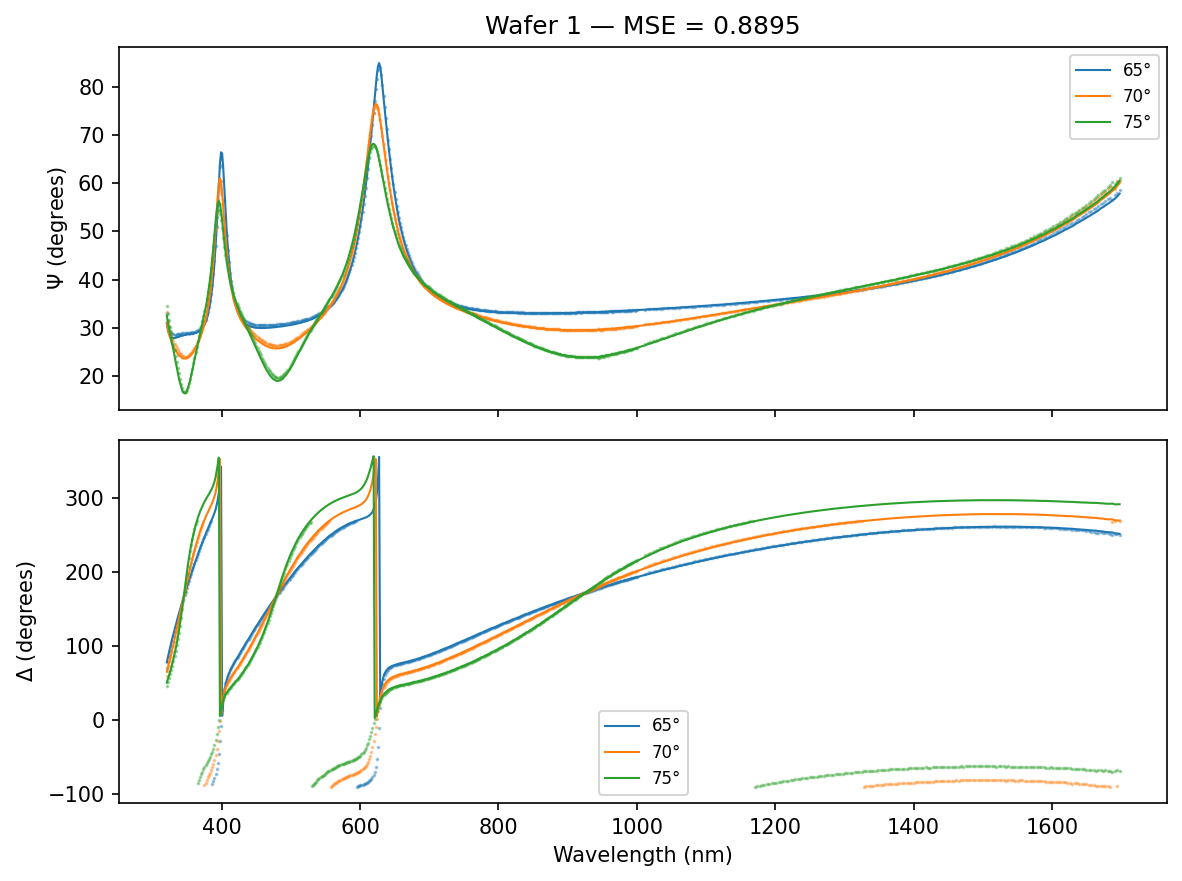
\includegraphics[width=0.85\textwidth]{fit_wafer_1_01242007.png}
\caption{Wafer 1 fit: $\Psi$ and $\Delta$ vs.\ wavelength at 65\textdegree, 70\textdegree, 75\textdegree.}
\label{fig:wafer1}
\end{figure}

\begin{figure}[H]
\centering
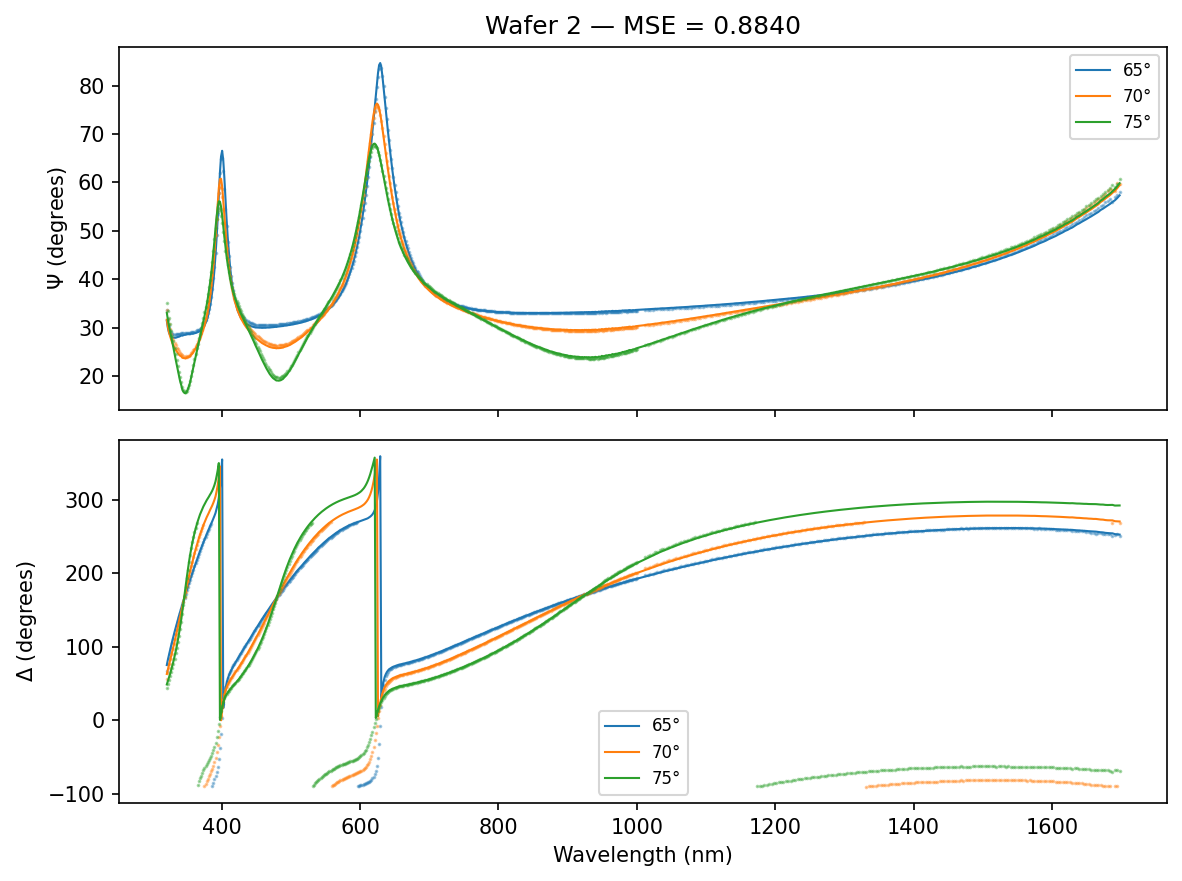
\includegraphics[width=0.85\textwidth]{fit_wafer_2_01242007.png}
\caption{Wafer 2 fit: $\Psi$ and $\Delta$ vs.\ wavelength at 65\textdegree, 70\textdegree, 75\textdegree.}
\label{fig:wafer2}
\end{figure}

\begin{figure}[H]
\centering
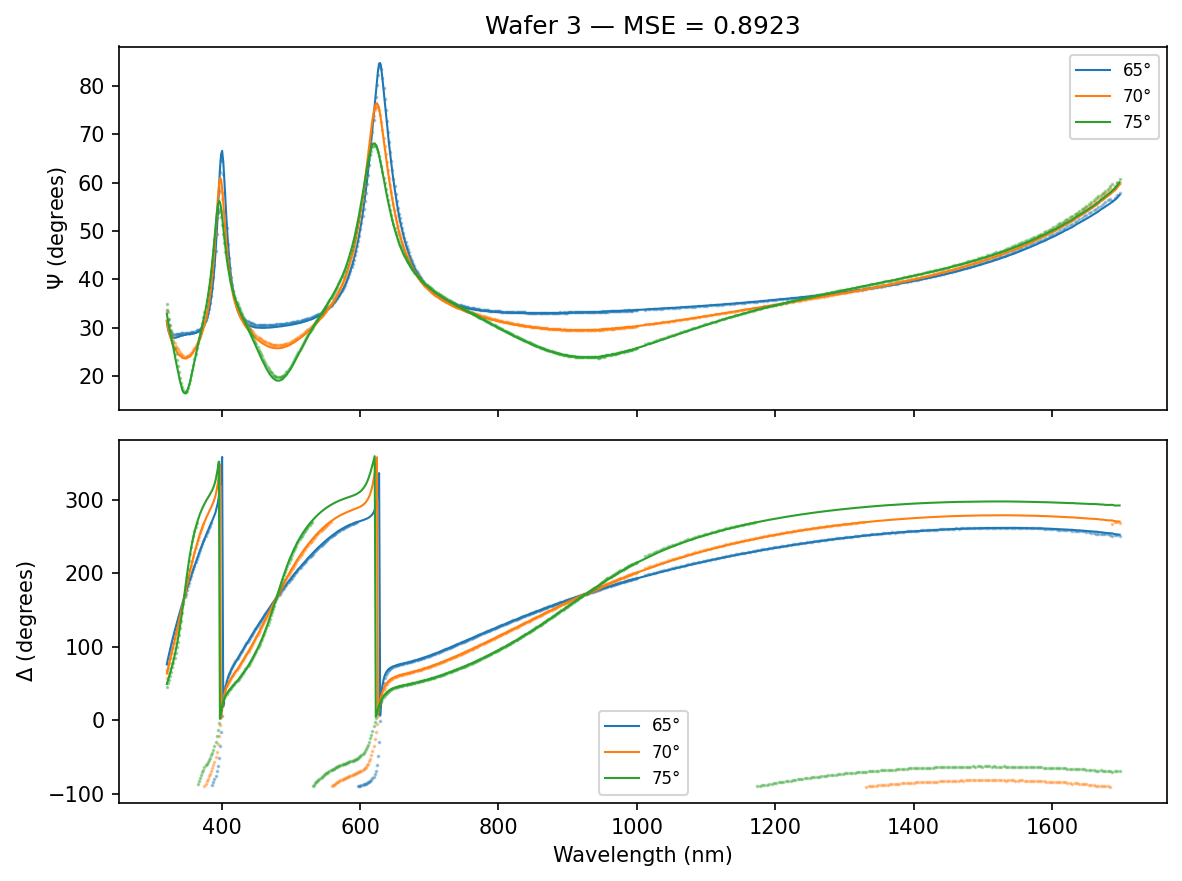
\includegraphics[width=0.85\textwidth]{fit_wafer_3_01242007.png}
\caption{Wafer 3 fit: $\Psi$ and $\Delta$ vs.\ wavelength at 65\textdegree, 70\textdegree, 75\textdegree.}
\label{fig:wafer3}
\end{figure}

\begin{figure}[H]
\centering
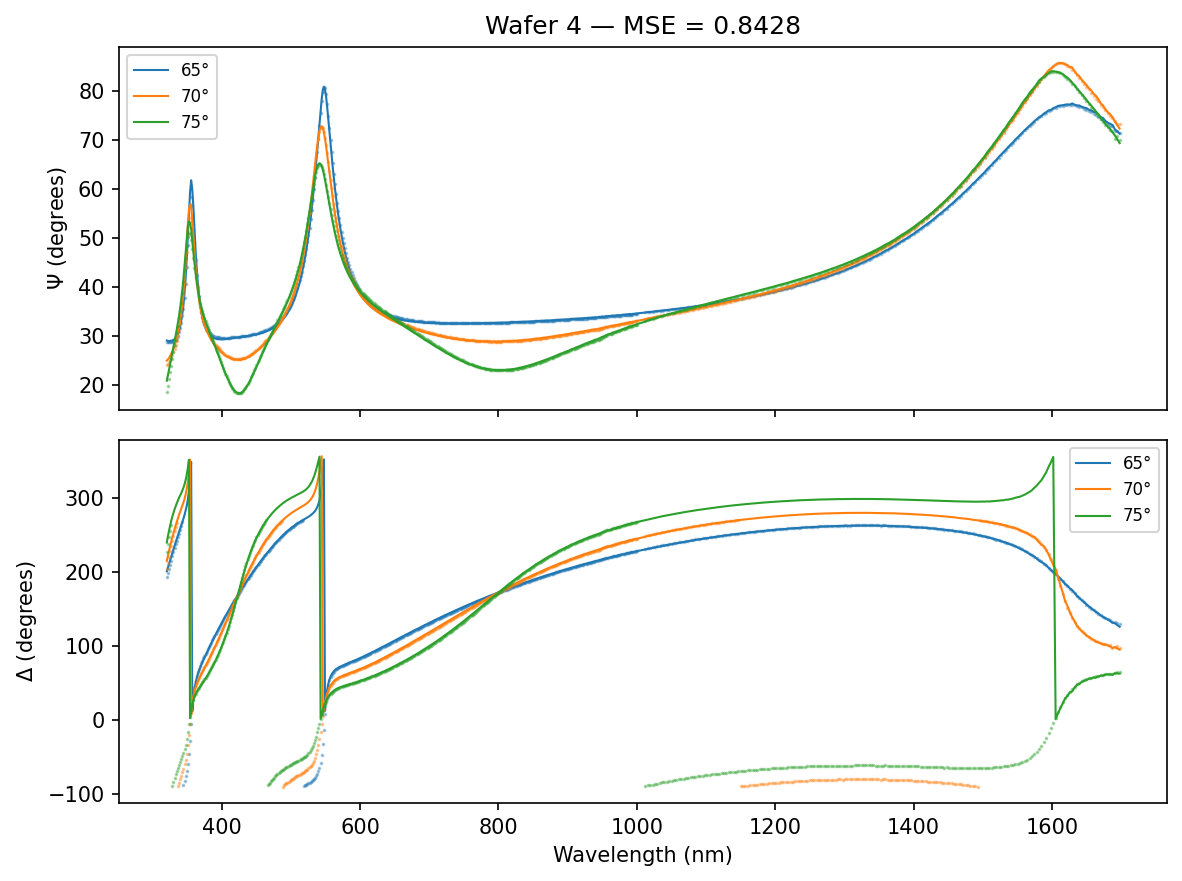
\includegraphics[width=0.85\textwidth]{fit_wafer_4_01242007.png}
\caption{Wafer 4 fit: $\Psi$ and $\Delta$ vs.\ wavelength at 65\textdegree, 70\textdegree, 75\textdegree.}
\label{fig:wafer4}
\end{figure}

\begin{figure}[H]
\centering
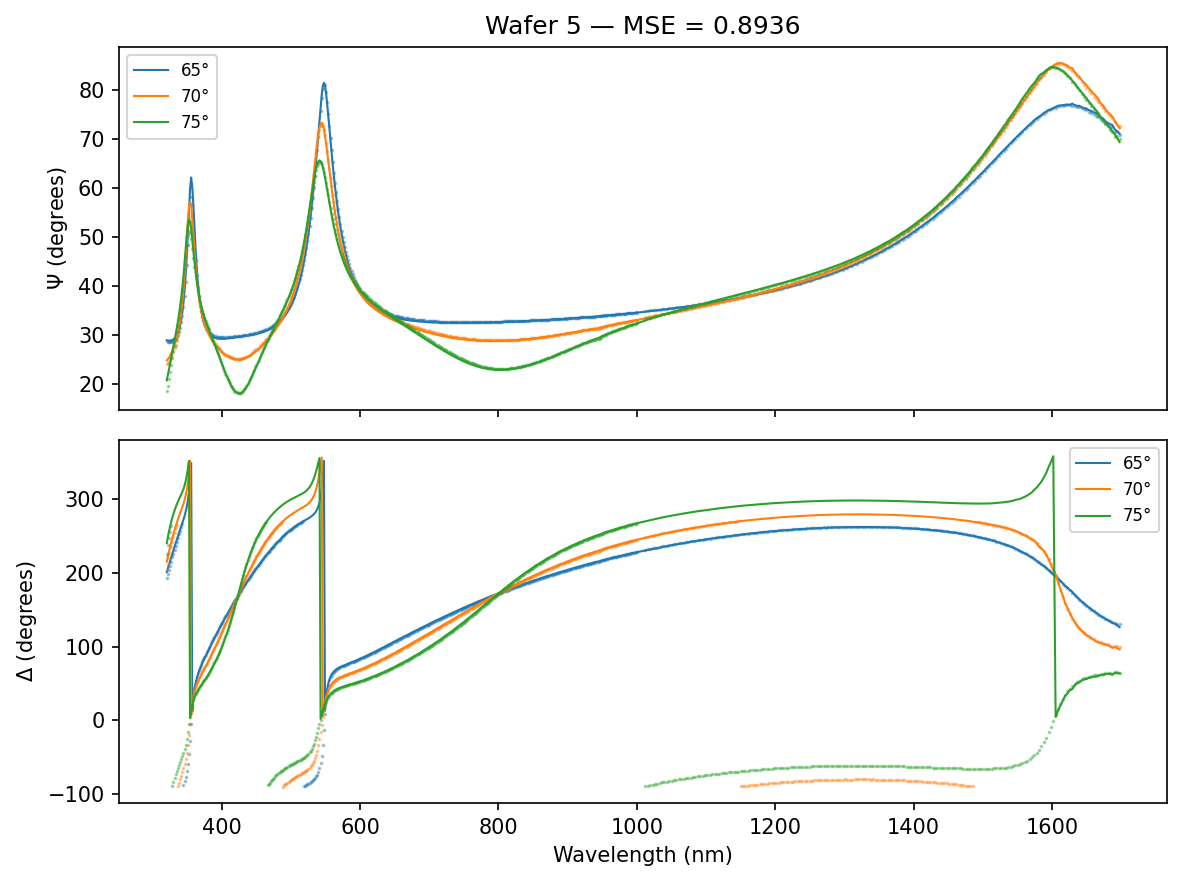
\includegraphics[width=0.85\textwidth]{fit_wafer_5_01242007.png}
\caption{Wafer 5 fit: $\Psi$ and $\Delta$ vs.\ wavelength at 65\textdegree, 70\textdegree, 75\textdegree.}
\label{fig:wafer5}
\end{figure}

\begin{figure}[H]
\centering
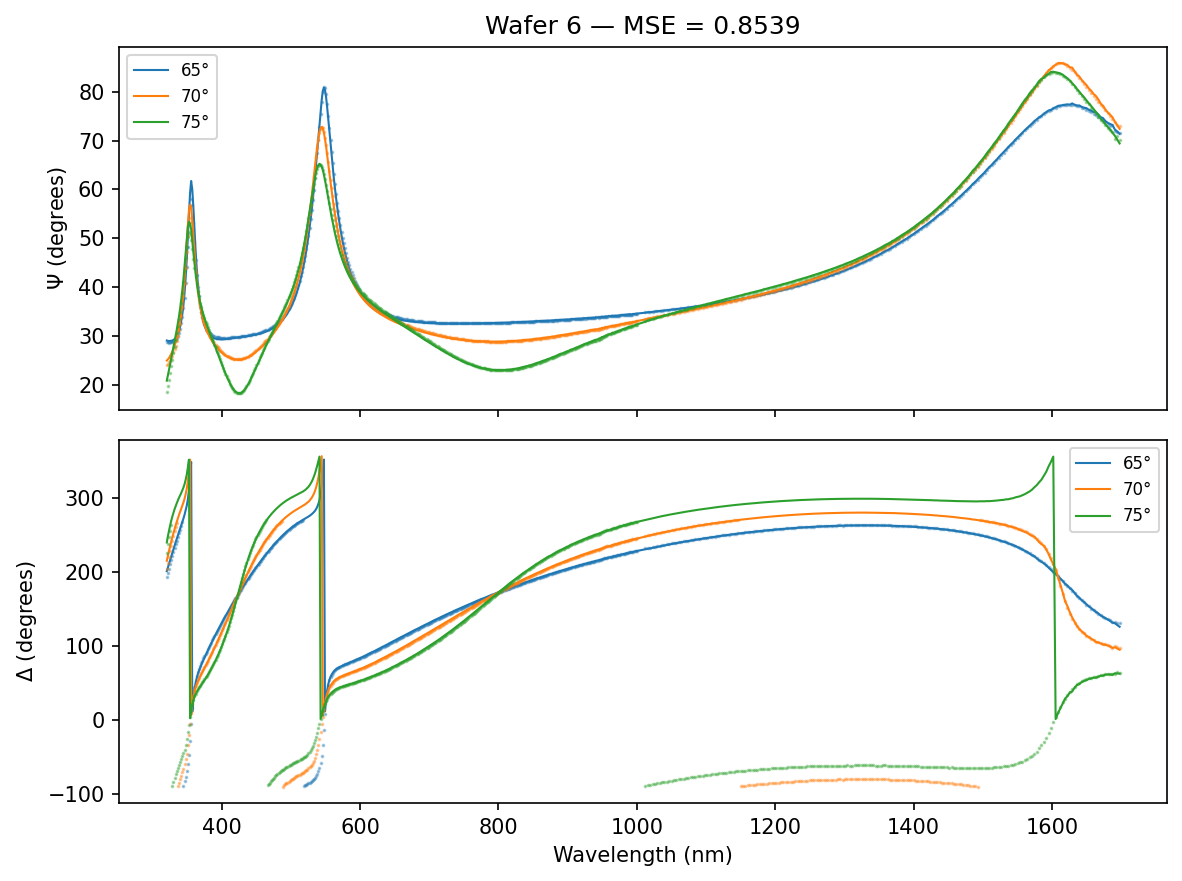
\includegraphics[width=0.85\textwidth]{fit_wafer_6_01242007.png}
\caption{Wafer 6 fit: $\Psi$ and $\Delta$ vs.\ wavelength at 65\textdegree, 70\textdegree, 75\textdegree.}
\label{fig:wafer6}
\end{figure}

\section{Discussion}

The two wafer groups (1--3 and 4--6) likely correspond to different process conditions
(noted as ``high current high voltage'' in the data headers). The thicker oxide in
wafers 1--3 suggests a longer or more aggressive oxidation, while the higher void fraction
in the EMA layer indicates a more porous interface.

The EMA void fraction for wafers 1--3 reaches $\sim$99\%, hitting the upper bound.
This suggests the interfacial layer is almost entirely roughness/air rather than
a graded composition layer. For wafers 4--6, the $\sim$84\% void fraction is more
physically reasonable and aligns with the original finding of $>80\%$ void.

The EMA layer thickness for wafers 4--6 hits the upper fitting bound (20\,nm),
suggesting the bound could be relaxed for further investigation. TEM microscopy
is recommended to validate the interfacial structure.

\section{Conclusion}

Neha Singh's model (Cauchy Ta\textsubscript{2}O\textsubscript{5} + EMA interfacial layer
+ Ta metal PBP substrate) provides excellent fits (MSE $< 0.9$) for all six wafers in
the Cap\_01242007 dataset. The porous interfacial layer is consistent with the columnar
grain roughness mechanism proposed by Curt.

\end{document}
